\documentclass[12pt,a4paper]{article}
\usepackage{tpl}
\dbegin{Геометрия, школа 179}{Новое доказательство формулы объёма пирамиды}

Итак, мы хотим доказать, что для произвольной пирамиды $V=\frac{1}{3}Sh$. Сразу же отметим, что достаточно доказывать это утверждение для пирамиды с любым фиксированным основанием площади $S$. Действительно, площади сечений этих пирамид плоскостями, параллельными основанию, будут равны, а значит, по принципу Кавальери равны и объёмы.

\begin{figure}[!htb]
	\begin{minipage}{0.96\textwidth}\centering
		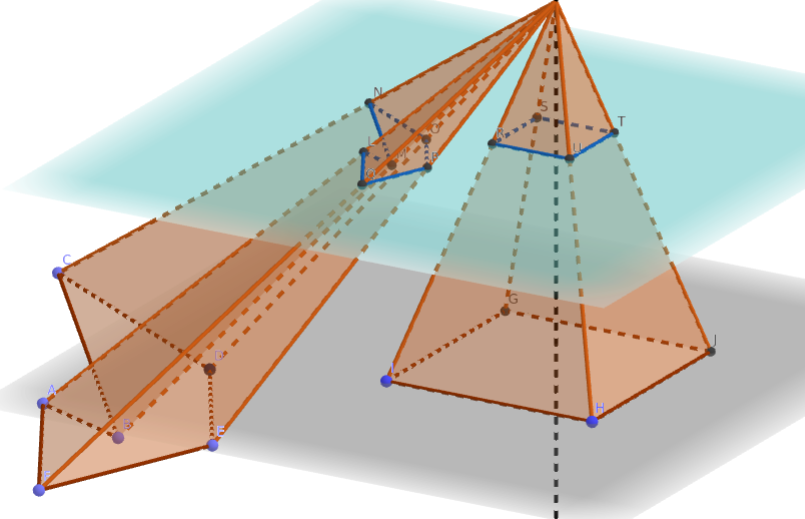
\includegraphics[scale=0.8]{kavalieri-pyramid-1.png}
	\end{minipage}
\end{figure}

Мы будем доказывать это утверждение для пирамид с прямоугольным основанием (например, можно взять как основание прямоугольник $1\times S$). Заметим, что параллелепипед объёма $2Sh$ можно разрезать на шесть прямоугольных пирамид с общей вершиной, которая совпадает с центром параллелепипеда. Дальше мы докажем, что объёмы этих пирамид будут равны.

\begin{figure}[!htb]
	\begin{minipage}{0.96\textwidth}\centering
		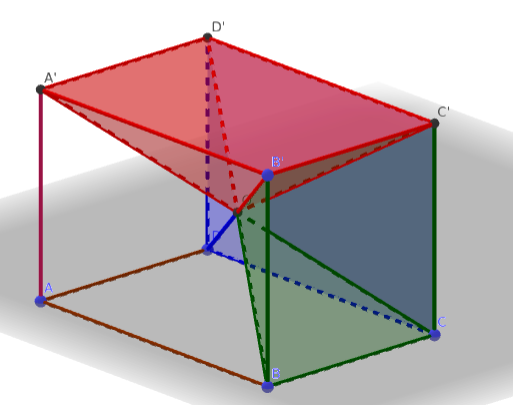
\includegraphics[scale=0.3]{kavalieri-pyramid-2.png}
	\end{minipage}
\end{figure}

Осталось доказать, что три пирамиды на рисунке выше (красная, синяя и зелёная) равновелики. И это снова можно сделать принципом Кавальери! Например, докажем, что зелёная пирамида равновелика красной. Каждое сечение каждой из этих пирамид плоскостью, параллельной $(A'BCD')$, это равнобокая трапеция (возможно, вырожденная --- треугольник или отрезок) и в силу симметрии относительно $XY$ --- пересечения нашей плоскости с $(AB'C'D)$ --- они равны, а значит, равновелики!

\begin{figure}[!htb]
	\begin{minipage}{0.96\textwidth}\centering
		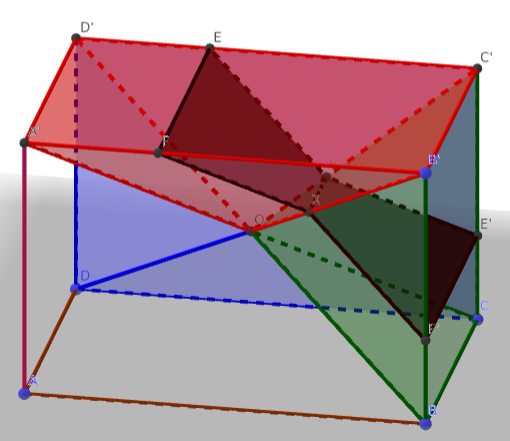
\includegraphics[scale=1]{kavalieri-pyramid-3.png}
	\end{minipage}
\end{figure}

Получается, эти две пирамиды --- красная и зелёная --- равновелики, а значит, и все 6 пирамид деления параллелепипеда равновелики. Но их суммарный объём равен $2Sh$, значит, объём каждой отдельно взятой пирамиды --- $\frac{1}{3}Sh$.\QEDA

\end{document}
